\documentclass[border=2mm]{standalone}

\usepackage{pgfplots}
\pgfplotsset{compat=1.18}
\usetikzlibrary{arrows.meta, calc, positioning, decorations.pathreplacing, calligraphy}

\usepackage{xcolor}
\definecolor{den-1}{HTML}{111111}   % Đen #111111
\definecolor{den-2}{HTML}{222222}   % Đen #222222
\definecolor{den-3}{HTML}{333333}   % Đen #333333
\definecolor{den-4}{HTML}{444444}   % Đen #444444
\definecolor{den-5}{HTML}{555555}   % Đen #555555
\definecolor{den-6}{HTML}{666666}   % Đen #666666

\tikzset{
  >=Stealth,
  originlabel/.style={
    font=\small\sf,
    anchor=north east, 
    yshift=-0.1ex,     
    xshift=-0.1ex      
  }
}

\begin{document}

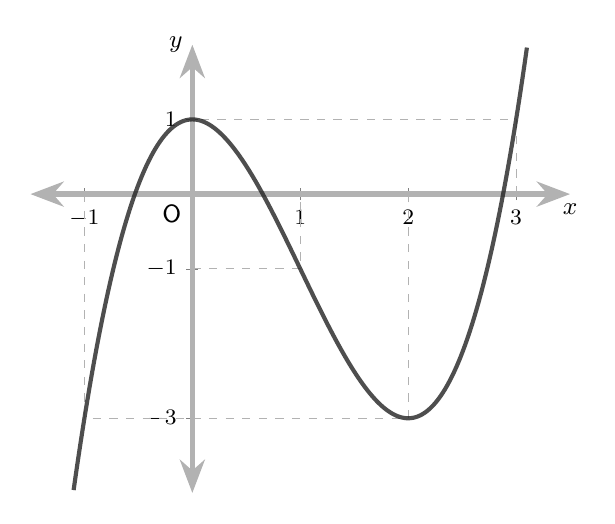
\begin{tikzpicture}

\begin{axis}[
    font=\small\sf,
    axis lines=middle,
    axis line style={<->, line width=2pt, color=den-6!50},
    xlabel=$x$, ylabel=$y$,
    xlabel style={below, font=\small\sf},
    ylabel style={left, font=\small\sf},
    xmin=-1.5, xmax=3.5,
    ymin=-4, ymax=2,
    xtick={-1,1,2,3},
    ytick={-3,-1,1},
    tick label style={font=\footnotesize\sf},
    clip=false,
]

\node[originlabel] at (axis cs:0,0) {O};

\draw [dashed, color=den-6!50] (-1,0) -- (-1,-3) -- (2,-3) -- (2,0);
\draw [dashed, color=den-6!50] (0,-1) -- (1,-1) -- (1,0);
\draw [dashed, color=den-6!50] (3,0) -- (3,1) -- (0,1);

\addplot[domain=-1.1:3.1, samples=200, line width=1.5pt, color=den-2, opacity=.8] {x^3 - 3*x^2 + 1};

\end{axis}

\end{tikzpicture}

\end{document}
